\section{\sysname{} Design}
\label{sec:system}

\sysname{} avoids the problems with manual policies or application-specific
solutions by structuring adaptation as a set of approximate, modular and
extensible specifications, or APIs (\autoref{sec:struct-adapt}). The
well-defined structure allows us to build a generic profiling tool that learns
an accurate relationship (the profile) between bandwidth consumption and
application accuracy (\autoref{sec:automatic-profiling}). The accurate profile
then allows the runtime to react with precision: achieving low latency and high
accuracy when facing bandwidth variation
(\autoref{sec:runtime}). \autoref{fig:overview} shows the high-level overview of
\sysname{}. We then discuss each stage in turn.

\begin{figure}
  \centering
  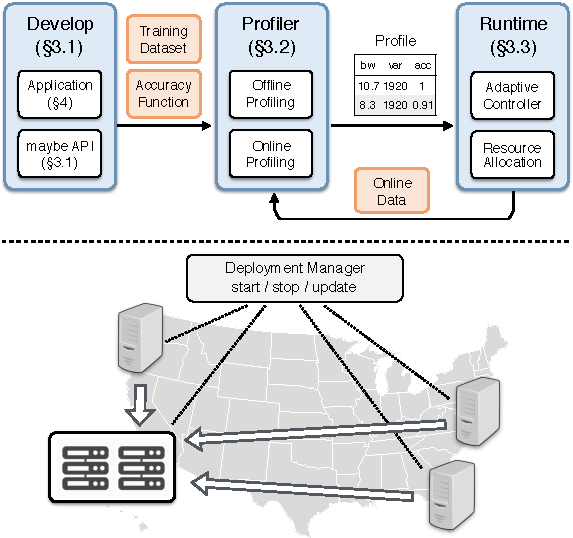
\includegraphics[width=.9\linewidth]{figures/system.pdf}
  \caption{High-level overview of \sysname{}.}
  \label{fig:overview}
\end{figure}

\subsection{APIs for Structured Adaptation}
\label{sec:struct-adapt}

%% Introduce graphs of operators model
The vast majority of stream processing applications today are constructed as a
directed graph of operators~\cite{toshniwal2014storm, zaharia2013discretized}).
\sysname{} employs such a programming model that integration with existing
applications will require minimal effort. \autoref{tab:operators} lists a few
example operators that \sysname{} supports.

In this model, each operator transforms existing streams into new
streams. Operators are specializable by user-defined functions (UDF). Optionally
developers can provide objects that implement a callable interface. Such objects
can be used to hold application states.

\begin{table*}
  \footnotesize
  \centering
  \begin{tabular}{ c r l }
    \toprule
    \multirow{7}{*}{Normal Operators}
    & \textit{map} (f: I $\Rightarrow$ O) & Stream<I> $\Rightarrow$ Stream<O> \\
    & \textit{skip} (i: Integer) & Stream<I> $\Rightarrow$
                                   Stream<I> \\
    & \textit{sliding\_window} (count: Integer, f: Vec<I> $\Rightarrow$ O) & Stream<I> $\Rightarrow$
                                                                            Stream<O> \\
    % & \textit{tumbling\_window} (count: Integer, f: Vec<I> $\Rightarrow$ O) & Stream<I> $\Rightarrow$
    %                                                                          Stream<O> \\
    & \textit{timed\_window} (time: Duration, f: Vec<I> $\Rightarrow$ O) & Stream<I> $\Rightarrow$
                                                                          Stream<O> \\
    & ... & ... \\
    \midrule
    \multirow{4}{*}{Degradation Operators}
    & \textit{maybe} (knobs: Vec<T>, f:  (T, I) $\Rightarrow$ I) & Stream<I> $\Rightarrow$
                                                                 Stream<I> \\
    & \textit{maybe\_skip} (knobs: Vec<Integer>) & Stream<I> $\Rightarrow$ Stream<I> \\
    & \textit{maybe\_downsample} (knobs: Vec<(Integer, Interger)>) & Stream<Image> $\Rightarrow$ Stream<Image> \\
    & ... & ... \\
    \bottomrule
  \end{tabular}
  \caption{A comparison between normal stream processing operators and our
    degradation operators. \texttt{Vec<T>} represents a list of elements of type
    T. \texttt{Option<T>} indicates an optional element of type T which is
    either present \texttt{Some(T)} or absent \texttt{None}.}
  \label{tab:operators}
\end{table*}

\sysname{} offers a special operator \texttt{maybe} to annotate degradation
operations. Developers use \texttt{maybe} with concrete operations that affect
the data size as well as data fidelity: these are the knobs tunable by the
system to explore performance trade-offs. The basic form of \texttt{maybe}
operator takes two arguments: a knob and a function. The knob is a vector of
values with type $T$ that encodes possible levels of degradation. The function
performs the actual operation. By default, the function needs to satisfy the
type constrain: $f(T, I) \Rightarrow I$. That is, only operations that does not
alter the type of the data stream are allowed. In this way, downstream operators
can work without the need to know if the degradation is in effect or not. A
relaxed version, \texttt{maybe\_with\_default}, exists for flexibility; but care
should be taken to use.

We illustrate the idea of \texttt{maybe} operator with an example that quantizes
a stream of integers in the Rust programming language. One possible
implementation is as follows:

\vspace{-2pt}
\begin{lstlisting}
    let quantized_stream = vec![1, 2, 3, 4].into_stream()
        .maybe(vec![2, 4], |k, p| p.wrapping_div(k));
        .collect();
\end{lstlisting}

The code creates a stream of integers [1, 2, 3, 4] and pass it through a
degradation operation. In this example, the knob is chosen as [2, 4]. The
degradation function performs a wrapping (modular) division where the divisor is
the knob. Depending on the quantization level, the output will be either [1, 2,
3, 4] (no degradation), [0, 1, 1, 2] (k=2), or [0, 0, 0, 1] (k=4). The
\texttt{collect} method will run this stream and hold the output in a vector.
If the stream is subsequently encoded (e.g. run-length encoding as in
JPEG~\cite{wallace1992jpeg}) for transmission, the data size will change
according to the level of degradation.

Based on the \texttt{maybe} primitive, one can implement wrappers for common
degradation operations. For example, \texttt{maybe\_skip} will optionally
subsample a stream; and \texttt{maybe\_downsample} can adjust the image
resolution to a configured target. \sysname{} provides a few such operations as
libraries for developers.

Using our APIs, the example mentioned in \autoref{sec:manual-policy} can now be
implemented as follows:

\vspace{-2pt}
\begin{lstlisting}[caption={Video Processing Example}, label={lst:ex}]
   let app = Camera::new((1920, 1080, 30))
      .maybe_downsample(vec![(1600, 900), (1280, 720)])
      .maybe_skip(vec![2, 5])
      .map(|frame| frame.show())
      .compose();
\end{lstlisting}

This snippet first instantiate a \texttt{Camera} source, which produces
\texttt{Stream<Image>} with 1920x1080 resolution and 30 FPS. Two degradation
operations are chained after the source: one that downsample the resolution to
either 1600x900 or 1280x720; the other skip the frame with a parameter of 2 or
5, resulting in 30/(2+1)=10 FPS or 30/(5+1)= 6 FPS. After the degradation,
images are shown on the display. In practice, further processing (such as
encoding and transmission) operators can be chained.

While \maybe{} itself has simplified the specification of degradation, the exact
level of degradation has to be known for precise rate adjustment at runtime. The
second stage of \sysname{} performs automatic profiling.

%%% Local Variables:
%%% mode: latex
%%% TeX-master: "sosp17"
%%% End:

\subsection{Automatic Profiling}
\label{sec:automatic-profiling}

After developers use \maybe{} operators to specify potential degradation
operations, \sysname{} automatically builds an accurate profile. The profile
captures the relationship between \textit{application accuracy} and \textit{bandwidth
consumption}
under different \textit{combinations} of data degradation operations. We describe the
formalism, followed by techniques that efficiently perform offline and online
profiling.

\para{Profiling formalism.} Suppose a stream processing application has $n$
\maybe{} operators. Each operator introduces a knob $k_i$ and their combination
forms a \textit{configuration} $c = [k_{1}, k_{2}, ... k_{n}]$. The set of all
possible configurations $\mathbb{C}$ is the space that the profiling
explores. For each configuration $c$, there are two mappings that are of
particular interest: a mapping from $c$ to its bandwidth consumption $B(c)$ and
its accuracy measure $A(c)$. \autoref{tab:notations} summarizes the notations
used in this paper.

The profiling looks Pareto-optimal configurations, that is, for any
configuration $c$ in the Pareto-optimal set, there is no alternative
configuration $c'$ that requires less bandwidth and offers a higher
accuracy. The Pareto-optimal set $\mathbb{P}$ is defined mathematically as
follows:

{\small \vspace{-1em}
  \begin{equation}
  \mathbb{P} = \{ c \in \mathbb{C} : \{ c' \in \mathbb{C}: B(c') < B(c),
  A(c') > A(c) \} = \varnothing\}
  \label{eq:pareto}
\end{equation}
}%

\begin{table}
  \footnotesize
  \centering
  \begin{tabular}{r l}
    \toprule
    \textbf{Symbol} & \textbf{Description} \\
    \midrule
    $n$ & number of degradation operations \\
    $k_i$ & the \textit{i}-th degradation knob \\
    $c = [k_{1}, k_{2}, ... k_{n}]$ & one specific configuration \\
    $\mathbb{C}$ & the set of all configurations \\
    \midrule
    $B(c)$ & bandwidth requirement for $c$ \\
    $A(c)$ & accuracy measure for $c$ \\
    $\mathbb{P}$ & Pareto-optimal set \\
    \midrule
    $c_i$, $c_{i+1}$, $c_{\max}$ & current/next/maximal configuration at runtime \\
    $R$ & network delivery rate (estimated bandwidth) \\
    $\text{Q}_\text{E}$, $\text{Q}_\text{C}$ & messages when \texttt{Queue} is empty or congested \\
    $\text{R}_\text{C}$ & message when \texttt{Receiver} detects congestion \\
    $\text{AC}_\text{Probe}$ & message when \texttt{AC} requests probing \\
    $\text{S}_\text{ProbeDone}$ & message when \texttt{Socket} finishes probing \\
    \bottomrule
  \end{tabular}
  \caption{Notations used in this paper.}
  \label{tab:notations}
\end{table}

Because \sysname{} allows arbitrary functions as the degradation functions, it
does not assume a closed-form relation for $B(c)$ and $A(c)$. Instead,
\sysname{} takes a data-driven approach: profiling applications with
developer-supplied training data.  We measure $B(c)$ at the point of
\textit{transmission}. The accuracy $A(c)$ is measured either against the \textit{ground-truth},
or the reference results when \textit{all degradation operations are off}.  We show
examples of concrete knobs, configurations, accuracy functions when we present
applications in \autoref{tab:apps}.

\para{Offline Profiling.} We first use an offline process to build a bootstrap
profile (or default profile).  \sysname{} makes no assumptions on the
performance models, and thus evaluate all possible configurations.  While all
knobs form a combinatorial space, the offline profiling is only a one-time
process.  We exploits parallelism to reduce the profiling time.  Without any
\textit{a priori} knowledge, all configurations are assigned randomly to
available machines.

% \para{Offline Profiling.} We first use an offline process to build a bootstrap
% profile (or default profile).  Because \sysname{} supports arbitrary
% degradation operations, we need to evaluate all combinations of the
% configurations offline profiling is a one-time process, \sysname{} currently
% performs an exhaustive evaluation of all configurations in $\mathbb{C}$
% despite all knobs form a combinatorial space. Future work could explore
% statistical methods to build performance models with a smaller number of
% training samples~\cite{venkataraman2016ernest, alipourfard2017cherrypick}.
% \sysname{} exploits parallelism when profiling all configurations.  Without
% any \textit{a priori} knowledge, all configurations are assigned randomly to
% all available machines.

\para{Online Profiling:} \sysname{} runs an online profiling process
continuously to refine the profile. The refinement handles \textit{model
  drifts}, a problem when the learned profile fails to predict the performance
accurately. There are two challenges with online profiling.  $(i)$~There is no
ground-truth labels or reference data to compute accuracy. Because labelling
data is prohibitively labor intensive and time
consuming~\cite{russell2008labelme}, \sysname{} currently uses \textit{raw data as
the
reference}. At runtime, if the application streams raw data, the data is used for
online profiling. Otherwise, we allocate additional bandwidth to back-haul raw
data, but only do so when there is spare capacity. $(ii)$~Exhaustive profiling
is expensive. If the profiling takes too much time, the newly-learned profile
may already be stale. \sysname{} uses a combination of parallelism and sampling
techniques to speed up this process, as below:

\begin{itemize}[leftmargin=*, topsep=0pt, itemsep=0pt]

\item Parallelization with degradation-aware scheduling. Evaluating each
  configuration takes a different amount of time. Typically, an increase in the
  level of degradation leads to a decrease in computation; for example, a
  smaller FPS means fewer images to process. Therefore, we collect processing
  times for each configuration from the offline process and schedule online
  profiling with longest first schedule (LFS)~\cite{karger2010scheduling} during
  parallelization.

\item Sampling-based profiling. Online profiling can speed up if we only profile
  a subset of all data or a subset of all configurations.  Sampling data reduces
  the amount of data to process, but at a cost of generating less accurate
  profiles. When sampling configuration, we can evaluate a subset of the
  Pareto-optimal configurations and compare their performances with the existing
  profile. A substantial difference, such as more than 1 mbps of bandwidth
  estimation, triggers a full profiling over all configurations to update the
  current profile.

\end{itemize}

%%% Local Variables:
%%% mode: latex
%%% TeX-master: "awstream"
%%% End:

\subsection{Runtime Adaptation}
\label{sec:runtime}

At runtime, \sysname{} performs application adaptation according to the learned
profile. We choose to design our own runtime system and adaptation algorithm
because prior solutions are not satisfactory: $(i)$~network protocols adapt to
available resources without application accuracy guarantee; $(ii)$
JetStream~\cite{rabkin2014aggregation} uses manual policies and doesn't support
degradations along multiple dimensions; and $(iii)$~video streaming adaptation,
such as Huang et al.~\cite{huang2014buffer}, uses the playback buffer and incurs
high latency.

Our runtime differs from prior systems in the ability to react
with precision: it stays in a low-latency state and uses a Pareto-optimal
configuration for high accuracy.

\begin{figure}
  \centering
  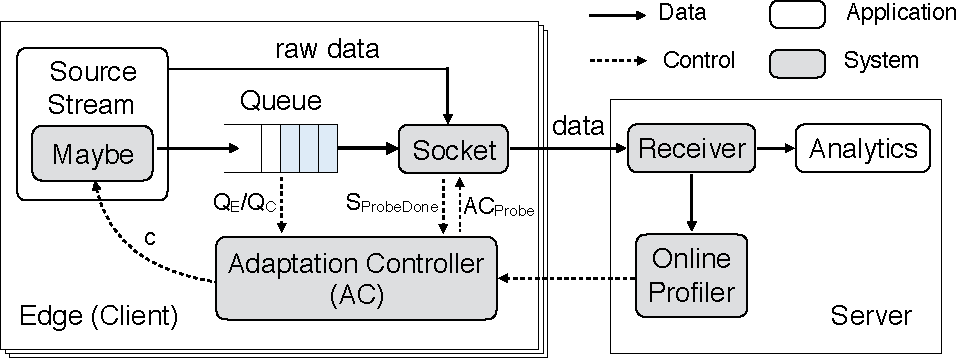
\includegraphics[width=\linewidth]{figures/runtime-adaptation.pdf}
  \caption{Runtime adaptation system architecture.}
  \label{fig:runtime}
\end{figure}

\autoref{fig:runtime} shows our runtime system architecture. \sysname{}
applications' source contains a \texttt{Maybe} module derived from all \maybe{}
operations. This module allows the controller to update the level of
degradation. Data generated by the source is then enqueued to \texttt{Queue} and
subsequently dequeued by \texttt{Socket}. When the data generation rate exceeds
\texttt{Socket}'s departure rate, the queue grows. In this case, the adaptation
controller (AC) queries the estimated bandwidth from \texttt{Socket} and
regulates the source stream by updating the configuration.  After the data is
sent through the network, the receiver extracts raw data to the online profiler
and delivers data to the application analytics. Raw data is only transmitted
when the queue is empty. When a new profile is learned, it is fed back to AC for
subsequent adaptation.

We then describe the adaptation algorithm; \autoref{fig:cc} shows the state
machine model and an example trace for illustration.  AC loads the profile and
sorts all configurations with an ascending order of bandwidth demand, resulting
in a list $[c_1, \dots, c_{\max}]$.  These configurations follow a total order:
$c_i < c_j$ if $B(c_i) < B(c_j)$.  We denote the current configuration as $c_i$
and the next $c_{i+1}$.  AC receives messages from the \texttt{Queue}: message
\qe{} when the queue is empty and $\text{Q}_\text{C}$ when queued items exceed a
threshold. AC can query \texttt{Socket} for delivery rate $R$ or request it to
probe ($\text{AC}_{\text{Probe}}$) for a target bandwidth, often
$B(c_{i+1})$. When $R > B(c_{i+1})$, \texttt{Socket} sends back \spd{}. The
algorithm follows a state machine as described below:

\begin{itemize}[leftmargin=*, topsep=3pt, itemsep=0pt]

\item \textbf{Startup: rapid growth.} \sysname{} starts with $c_1$ and grows the
  rate ($c_i \Rightarrow c_{i+1}$) upon each \qe{}. The growth stops at
  $c_{\max}$ (to \texttt{Steady}) or if it receives \qc{} (to \texttt{Degrade}).

\item \textbf{Degrade: reacting to congestion.} When \texttt{Queue} grows and
  exceeds a threshold, AC receives \qc{} and runs the \texttt{adapt()}
  procedure. This involves two steps: (1) AC queries $R$ from \texttt{Socket};
  (2) AC updates \texttt{Maybe} with the maximum-allowed $c$ that satisfies
  $B(c) < \alpha R, \alpha \in (0, 1)$. A smaller $\alpha$ allows a quicker
  draining of the queue. After the queue is drained, \sysname{} changes to
  \texttt{Steady}.

\item \textbf{Steady: low latency delivery.} \sysname{} achieves low latency by
  spending most of the time in the \texttt{Steady} state. It changes to
  \texttt{Degrade} when congestion occurs. If $c < c_{\max}$ and it receives
  \qe{}, AC enters the \texttt{Probe} state to check for more available
  bandwidth.

\item \textbf{Probe: more bandwidth for a higher accuracy.} Advancing the configuration
  directly causes a drastic latency increase when $B(c_{i+1}) \gg B(c_i)$. To
  allow a smooth increase, AC requests \texttt{Socket} to probe by sending
  additional traffic controlled by \texttt{probe\_gain} (in
  \texttt{inc\_pace()}, similar to BBR~\cite{cardwell2017bbr}). \sysname{} stops
  probing under two conditions: (1) upon \spd{}, it advances $c_i$; (2) upon
  \qc{}, it returns to \texttt{Steady}.

\end{itemize}

\begin{figure}
  \begin{subfigure}[t]{\columnwidth}
    \centering
    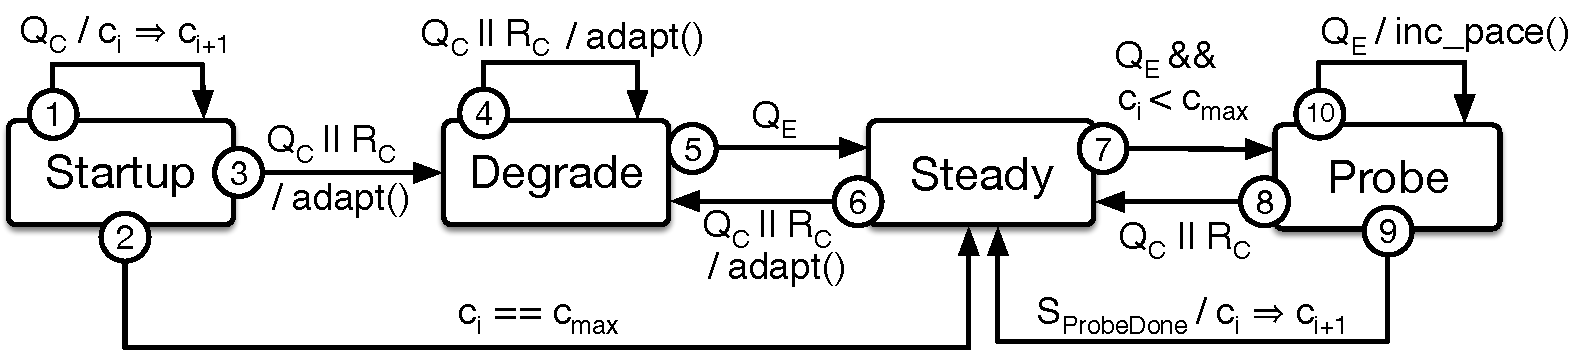
\includegraphics[width=\columnwidth]{figures/cc.pdf}
    \caption{Rate adaptation as a state machine.}
    \vspace{1em}
    \label{fig:cc-sm}
  \end{subfigure}
  \begin{subfigure}[t]{\columnwidth}
    \centering
    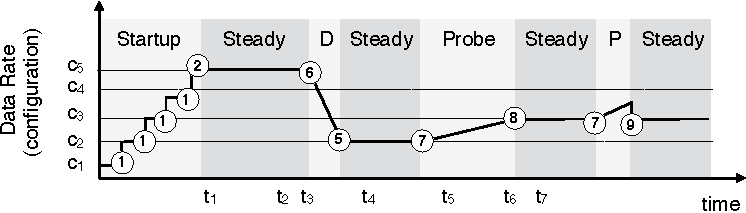
\includegraphics[width=\columnwidth]{figures/cc2.pdf}
    \caption{An example illustrating the adaptation algorithm.}
    \label{fig:cc-ex}
  \end{subfigure}
  \caption{Runtime adaptation algorithm.}
  \label{fig:cc}
\end{figure}

% \begin{figure}
%   \centering
%   \resizebox{\columnwidth}{!}{
%     \begin{tikzpicture}[
  state/.style = { draw, very thick, fill=white, rounded corners=1em,
    minimum height=3em, minimum width=7em, node distance=7em, font={\bfseries},
    align=center },
  edge portion/.style = { black, thick },
  transition/.style = { edge portion, -> },
  algorithm/.style = { draw, thin, fill=white },
  ]

  \node [state] (startup) {
    STARTUP };
  \node [state] (congestion) [right=of startup] {CONGESTION};
  \draw [transition] (startup) -- (congestion)
  node [midway, auto] {Q.Congestion};

  \node [state] (steady) [below=of congestion] {STEADY};

  \draw [transition] ($(congestion.south west)!0.4!(congestion.south east)$)
  to node[midway, sloped, below] {Q.NoQueue}
  ($(steady.north west)!0.4!(steady.north east)$);

  \draw [transition] ($(steady.north west)!0.6!(steady.north east)$)
  to node[midway, sloped, below] {Q.Congestion}
  ($(congestion.south west)!0.6!(congestion.south east)$);

  \node [state] (probe) [left=of steady] {PROBE};

  \draw [transition] ($(steady.south west)!0.6!(steady.north west)$)
  -- ($(probe.south east)!0.6!(probe.north east)$)
  node[midway, auto, swap] {Q.Probe};

  \draw [transition, <-] ($(steady.south west)!0.4!(steady.north west)$)
  -- ($(probe.south east)!0.4!(probe.north east)$)
  node[midway, auto, align=left] {Q.Congestion | \\ IO.ProbeDone};

\end{tikzpicture}


%%% Local Variables:
%%% mode: latex
%%% TeX-master: "sosp17"
%%% End:

%   }
%   \caption{Congestion Control Algorithm}
%   \label{fig:cc}
% \end{figure}

\para{Resource Allocation and Fairness.} In addition to rate adaptation, the
profile is also useful for controlling a single application's bandwidth usage or
allocating resources among competing tasks.

For individual applications, developers can pinpoint a configuration for a given
bandwidth or accuracy goal. They can also specify a criterion to limit effective
configurations. For example, \sysname{} can enforce an upper bound on the
bandwidth consumption, useful to reduce WAN bandwidth usage and cost.

For multiple applications, their profiles allows novel bandwidth allocation
schemes such as utility fairness. Different from traditional resource fairness
where applications get equal share of bandwidth, utility fairness aims
to maximize the \textit{minimal} application accuracy. With the profiles,
finding allocations is equivalent to finding proper configuration $c^t$ for
application $t$. We formulate utility fairness as follows:

%% Pick one based on the space

\begin{equation}
 \label{eq:multitask}
 \underset{c^t}{\max} \; \min({A^t(c^t)})
 \;
 \text{s.t.}
 \;
 \sum_t{B^t(c^t)} < R
\end{equation}

% \begin{equation}
%  \label{eq:multitask}
%  \begin{aligned}
%     & \underset{c^t}{\text{maximize}} & & \min({A^t(c^t)}) & & \\
%     & \text{subject to} & & \sum_t{B^t(c^t)} < R & & \\
%  \end{aligned}
% \end{equation}

Solving this optimization is computationally hard. \sysname{} uses a heuristics
approach. We start with $c_1^t$ and improve the application $t$ that has the
worst accuracy. This process repeats until we have allocated all available
bandwidth.

%%% Local Variables:
%%% mode: latex
%%% TeX-master: "awstream"
%%% End:


\newpage
\clearpage

%%% Local Variables:
%%% mode: latex
%%% TeX-master: "sosp17"
%%% End:
